%=========================================
% 	  Implementierung     		 =
%=========================================

\chapter{Implementierung}

In diesem Kapitel wird das Datenbank-Schema gezeigt und erkl"art, sowie der Quellcode der SQL-Anweisungen.\\

\section{Datenbank-Schema}
Es gibt in der Datenbank 2 Tables und 2 Views. Diese sind in ihren entsprechenden Dimensionen unterteilt. Die Tabeles embeddings\underline{  }100 und embeddings\underline{ }50 werden f"ur die SQL-Anweisung ben"otigt, die die Euklidische Distanz berechnet. Die Views Liste\underline{ }L"ange\underline{ }100 und Liste\underline{ }L"ange\underline{ }50 werden ben"otigt um f"ur die SQL-Anweisung der Kosinus "Ahnlichkeit die Formel zu vereinfachen, da man f"ur die Koninus "Ahnlichkeit die L"ange braucht.

\begin{figure}[bth] 
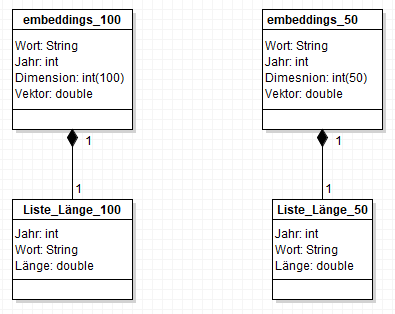
\includegraphics{Graphics/Datenbank.png}
\caption[Datenbank-Schema]{Struktur der Datenbank}
\end{figure}


\section{Quellcode}

\subsection{Euklidische Disntanz}
\begin{lstlisting}[style=Java]
public String selectEuklidisch(String wort1, int jahr1, int jahr2) throws SQLException {
        Statement statement = connection.createStatement();
        String wort = null;
        String sim = null;
        StringBuilder stringBuilder = new StringBuilder();

        ResultSet rs = statement.executeQuery("SELECT e2.Wort, sqrt(sum(pow(e1.Vektor - e2.Vektor,2))) as sim" +
                " FROM " + TABLE + " e1 , " + TABLE + " e2" +
                " WHERE e1.Wort='" + wort1 + "' AND e1.Jahr=" + jahr1 + " AND e2.Jahr=" + jahr2 + " AND e1.Dimension = e2.Dimension" +
                " GROUP BY e2.Wort" +
                " ORDER BY sim ASC" +
                " LIMIT 50 ");

        while (!rs.isLast()) {
            if (rs.next()) {
                wort = rs.getString(1);
                sim = rs.getString(2);
                stringBuilder.append(wort + ", ").append(sim).append("\n");
            }
        }

        return stringBuilder.toString();
    }
\end{lstlisting}


\subsection{Kosinus "Ahnlichkeit}
\begin{lstlisting}[style=Java]
public String selectCosinus(String wort1, int jahr1, int jahr2) throws SQLException {
        Statement statement = connection.createStatement();
        StringBuilder stringBuilder = new StringBuilder();
        String wort = null;
        String cos = null;


        ResultSet rs = statement.executeQuery("SELECT e2.Wort, sum(e1.Vektor * e2.Vektor) / (l1.Laenge * l2.Laenge) as cos" +
                " FROM " + TABLE + " e1 , " + TABLE + " e2 , " + VIEW + " l1 , " + VIEW + " l2" +
                " WHERE e1.Wort='" + wort1 + "' AND e1.Jahr=" + jahr1 + " AND e2.Jahr=" + jahr2 +
                " AND e1.Dimension=e2.Dimension AND e1.jahr=l1.jahr AND e2.jahr=l2.jahr AND l1.Wort=e1.Wort AND l2.Wort=e2.Wort" +
                " GROUP BY e2.Wort" +
                " ORDER BY cos DESC"+
                " LIMIT 100 ");

        while (!rs.isLast()) {
            if (rs.next()) {
                wort = rs.getString(1);
                cos = rs.getString(2);
                stringBuilder.append(wort + ", ").append(cos).append("\n");
            }
        }
        return stringBuilder.toString();
    }
\end{lstlisting}

\subsection{View erstellen}
\begin{lstlisting}[style=Java]
public void createView() throws SQLException {
        Statement statement = connection.createStatement();
        statement.executeUpdate("CREATE VIEW Liste_Laenge_50 ( Jahr, Wort, Laenge ) AS SELECT Jahr, Wort, sqrt(sum(Vektor * Vektor)) as Laenge" +
                " FROM embeddings_50"+
                " GROUP BY Jahr, Wort");
        statement.executeUpdate("CREATE VIEW Liste_Laenge_100 ( Jahr, Wort, Laenge ) AS SELECT Jahr, Wort, sqrt(sum(Vektor * Vektor)) as Laenge" +
                " FROM embeddings_100"+
                " GROUP BY Jahr, Wort");
    }
\end{lstlisting}

%Hier wird die Implementierung gezeigt und erklärt